\documentclass[journal,12pt,twocolumn]{IEEEtran}

\usepackage{setspace}
\usepackage{gensymb}
\singlespacing
\usepackage[cmex10]{amsmath}

\usepackage{amsthm}

\usepackage{mathrsfs}
\usepackage{txfonts}
\usepackage{stfloats}
\usepackage{bm}
\usepackage{cite}
\usepackage{cases}
\usepackage{subfig}

\usepackage{longtable}
\usepackage{multirow}

\usepackage{enumitem}
\usepackage{mathtools}
\usepackage{steinmetz}
\usepackage{tikz}
\usepackage{circuitikz}
\usepackage{verbatim}
\usepackage{tfrupee}
\usepackage[breaklinks=true]{hyperref}
\usepackage{graphicx}
\usepackage{tkz-euclide}

\usetikzlibrary{calc,math}
\usepackage{listings}
    \usepackage{color}                                            %%
    \usepackage{array}                                            %%
    \usepackage{longtable}                                        %%
    \usepackage{calc}                                             %%
    \usepackage{multirow}                                         %%
    \usepackage{hhline}                                           %%
    \usepackage{ifthen}                                           %%
    \usepackage{lscape}     
\usepackage{multicol}
\usepackage{chngcntr}

\DeclareMathOperator*{\Res}{Res}

\renewcommand\thesection{\arabic{section}}
\renewcommand\thesubsection{\thesection.\arabic{subsection}}
\renewcommand\thesubsubsection{\thesubsection.\arabic{subsubsection}}

\renewcommand\thesectiondis{\arabic{section}}
\renewcommand\thesubsectiondis{\thesectiondis.\arabic{subsection}}
\renewcommand\thesubsubsectiondis{\thesubsectiondis.\arabic{subsubsection}}


\hyphenation{op-tical net-works semi-conduc-tor}
\def\inputGnumericTable{}                                 %%

\lstset{
%language=C,
frame=single, 
breaklines=true,
columns=fullflexible
}
\begin{document}


\newtheorem{theorem}{Theorem}[section]
\newtheorem{problem}{Problem}
\newtheorem{proposition}{Proposition}[section]
\newtheorem{lemma}{Lemma}[section]
\newtheorem{corollary}[theorem]{Corollary}
\newtheorem{example}{Example}[section]
\newtheorem{definition}[problem]{Definition}

\newcommand{\BEQA}{\begin{eqnarray}}
\newcommand{\EEQA}{\end{eqnarray}}
\newcommand{\define}{\stackrel{\triangle}{=}}
\bibliographystyle{IEEEtran}
\raggedbottom
\setlength{\parindent}{0pt}
\providecommand{\mbf}{\mathbf}
\providecommand{\pr}[1]{\ensuremath{\Pr\left(#1\right)}}
\providecommand{\qfunc}[1]{\ensuremath{Q\left(#1\right)}}
\providecommand{\sbrak}[1]{\ensuremath{{}\left[#1\right]}}
\providecommand{\lsbrak}[1]{\ensuremath{{}\left[#1\right.}}
\providecommand{\rsbrak}[1]{\ensuremath{{}\left.#1\right]}}
\providecommand{\brak}[1]{\ensuremath{\left(#1\right)}}
\providecommand{\lbrak}[1]{\ensuremath{\left(#1\right.}}
\providecommand{\rbrak}[1]{\ensuremath{\left.#1\right)}}
\providecommand{\cbrak}[1]{\ensuremath{\left\{#1\right\}}}
\providecommand{\lcbrak}[1]{\ensuremath{\left\{#1\right.}}
\providecommand{\rcbrak}[1]{\ensuremath{\left.#1\right\}}}
\theoremstyle{remark}
\newtheorem{rem}{Remark}
\newcommand{\sgn}{\mathop{\mathrm{sgn}}}
\providecommand{\abs}[1]{\left\vert#1\right\vert}
\providecommand{\res}[1]{\Res\displaylimits_{#1}} 
\providecommand{\norm}[1]{\left\lVert#1\right\rVert}
%\providecommand{\norm}[1]{\lVert#1\rVert}
\providecommand{\mtx}[1]{\mathbf{#1}}
\providecommand{\mean}[1]{E\left[ #1 \right]}
\providecommand{\fourier}{\overset{\mathcal{F}}{ \rightleftharpoons}}
%\providecommand{\hilbert}{\overset{\mathcal{H}}{ \rightleftharpoons}}
\providecommand{\system}{\overset{\mathcal{H}}{ \longleftrightarrow}}
	%\newcommand{\solution}[2]{\textbf{Solution:}{#1}}
\newcommand{\solution}{\noindent \textbf{Solution: }}
\newcommand{\cosec}{\,\text{cosec}\,}
\providecommand{\dec}[2]{\ensuremath{\overset{#1}{\underset{#2}{\gtrless}}}}
\newcommand{\myvec}[1]{\ensuremath{\begin{pmatrix}#1\end{pmatrix}}}
\newcommand{\mydet}[1]{\ensuremath{\begin{vmatrix}#1\end{vmatrix}}}
\numberwithin{equation}{subsection}

\makeatletter
\@addtoreset{figure}{problem}
\makeatother
\let\StandardTheFigure\thefigure
\let\vec\mathbf

\renewcommand{\thefigure}{\theproblem}

\def\putbox#1#2#3{\makebox[0in][l]{\makebox[#1][l]{}\raisebox{\baselineskip}[0in][0in]{\raisebox{#2}[0in][0in]{#3}}}}
     \def\rightbox#1{\makebox[0in][r]{#1}}
     \def\centbox#1{\makebox[0in]{#1}}
     \def\topbox#1{\raisebox{-\baselineskip}[0in][0in]{#1}}
     \def\midbox#1{\raisebox{-0.5\baselineskip}[0in][0in]{#1}}
\vspace{3cm}
\title{Assignment 1}
\author{KRATI ARELA - EE18BTECH11050}
\maketitle
\newpage
\renewcommand{\thefigure}{\theenumi}
\renewcommand{\thetable}{\theenumi}



Download all C and python codes from 
\begin{lstlisting}
https://github.com/Krati012/EE3025/tree/main/Assignment1_C/codes
\end{lstlisting}
and latex-tikz codes from 
\begin{lstlisting}
https://github.com/Krati012/EE3025/tree/main/Assignment1_C
\end{lstlisting}
%%%%%%
\section{Digital Filter}
\begin{enumerate}[label=\thesection.\arabic*
,ref=\thesection.\theenumi]
\item
\label{prob:inp}
Download the sound file from  
\begin{lstlisting}
wget https://raw.githubusercontent.com/gadepall/ 
EE1310/master/filter/codes/Sound_Noise.wav
\end{lstlisting}

\item
\label{prob:out}
Write the python code for removal of out of band noise and execute the code.
\\
\solution
\lstinputlisting{./codes/remove_noise.py}
\end{enumerate}
%%%%%%%
\section{Difference equation}

\begin{enumerate}[label=\thesection.\arabic*,ref=\thesection.\theenumi]
\item
\label{prob:diffEq}
Write the difference equation of the above Digital filter obtained in problem \ref{prob:out}.
\\
\solution
\begin{equation}
\label{eq:eqn1}
 \sum _{m=0}^{M}a\brak{m}y\brak{n-m}=\sum _{k=0}^{N}b\brak{k}x\brak{n-k}
\end{equation}
\begin{equation}
\label{eq:eqn2}
\begin{split}
y(n) - 2.52y(n-1) + 2.56y(n-2) - 1.206y(n-3)
\\
+ 0.22013y(n-4) = 0.00345x(n) + 0.0138x(n-1)
\\
+ 0.020725x(n-2) + 0.0138x(n-3) + 0.00345x(n-4)
\end{split}
\end{equation}

\item
\label{prob:plot_x_y}
Sketch x(n) and y(n).
\\
\solution
The following code generates x(n) as x.dat file from .wav file
\begin{lstlisting}
codes/generateX.py
\end{lstlisting}

The following code computes $x(n)$ and $y(n)$ from the difference equation.
\begin{lstlisting}
codes/x_y.c
\end{lstlisting}
The following code plots $x(n)$ and $y(n)$ in Fig. \ref{fig:xy}
\begin{lstlisting}
codes/plot_xy.py
\end{lstlisting}
\begin{figure}[!ht]
\begin{center}
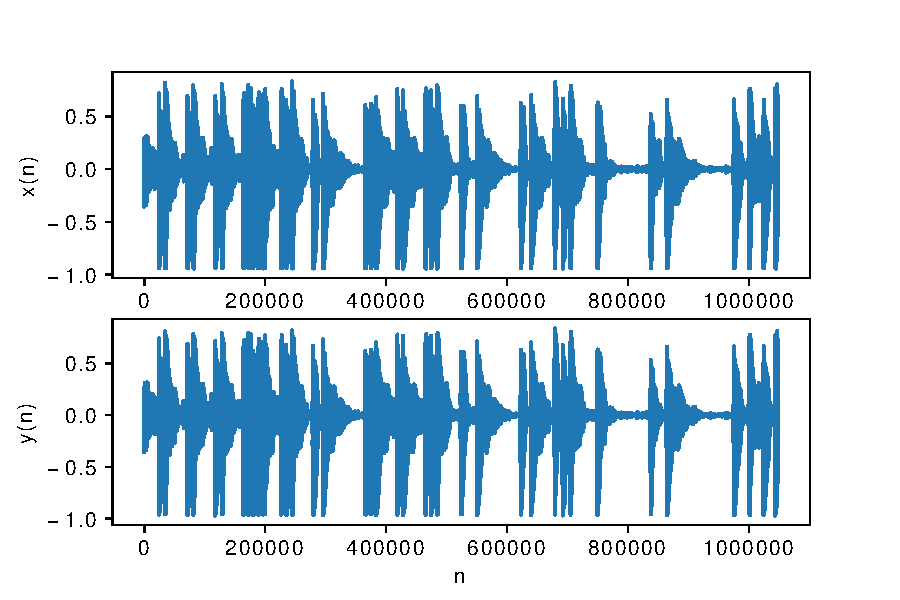
\includegraphics[width=\columnwidth]{./figs/xnyn}
\end{center}
\captionof{figure}{Digital Filter Input-Output}
\label{fig:xy}	
\end{figure}
\end{enumerate}

%%%%%%
\section{DFT and FFT}
\begin{enumerate}[label=\thesection.\arabic*
,ref=\thesection.\theenumi]
\item Compute
\begin{align}
        X(k) \triangleq \sum_{n=0}^{N-1} x(n) e^{-j 2 \pi k n / N}, \quad k=0,1, \ldots, N-1
\end{align}
and $H(k)$ using h(n).
\\
\solution
For this given IIR system with audio sample as x(n) and h(n) as impulse response 

DFT of Input Signal $x(n)$ is 
\begin{align}
    X(k) \triangleq \sum_{n=0}^{N-1} x(n) e^{-j 2 \pi k n / N}, \quad k=0,1, \ldots, N-1
\end{align}
DFT of Impulse Response $h(n)$ is 
\begin{align}
    H(k) \triangleq \sum_{n=0}^{N-1} h(n) e^{-j 2 \pi k n / N}, \quad k=0,1, \ldots, N-1
\end{align}

The following C code computes FFT of $x(n)$ and $h(n)$ using divide and conquer approach using recursive calls and saves the results in .dat file
\begin{lstlisting}
codes/fft.c
\end{lstlisting}
The following code plots FFT of $x(n)$ and $h(n)$ using .dat files obtained from the above code
\begin{lstlisting}
codes/plotFFT.py
\end{lstlisting}
Magnitude plots of $|X(k)|$ and $|H(k)|$ obtained through above code is in Fig. \ref{fig:fft}.
\begin{figure}[!ht]
\centering
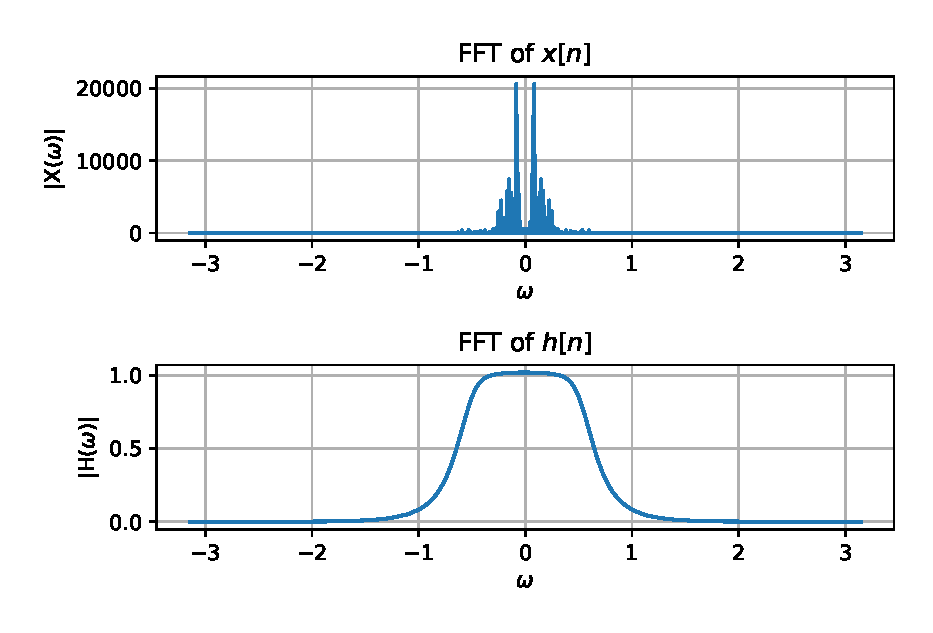
\includegraphics[width=\columnwidth]{./figs/fft}
\caption{$X(k)$ and $H(k)$}
\label{fig:fft}
\end{figure}
We can observe that these above plots look similar to the ones generated using the in-built FFT function.
\item From
\begin{equation}
Y(k) = X(k)H(k)
\end{equation}
compute
\begin{equation}
y(n) \triangleq \sum_{k=0}^{N-1} Y(k) e^{j 2 \pi k n / N}, \quad n=0,1, \ldots, N-1
\end{equation}
\\
\solution
The following C code computes $Y(k)$ by multiplying $X(k)$ and $H(k)$ and then computes IFFT to obtain $y(n)$
\begin{lstlisting}
codes/ifft.c 
\end{lstlisting}
The following code plots $y(n)$ in Fig.\ref{fig:ifft} from .dat obtained from above code
\begin{lstlisting}
codes/plotIFFT.py
\end{lstlisting}
\begin{figure}[!ht]
\centering
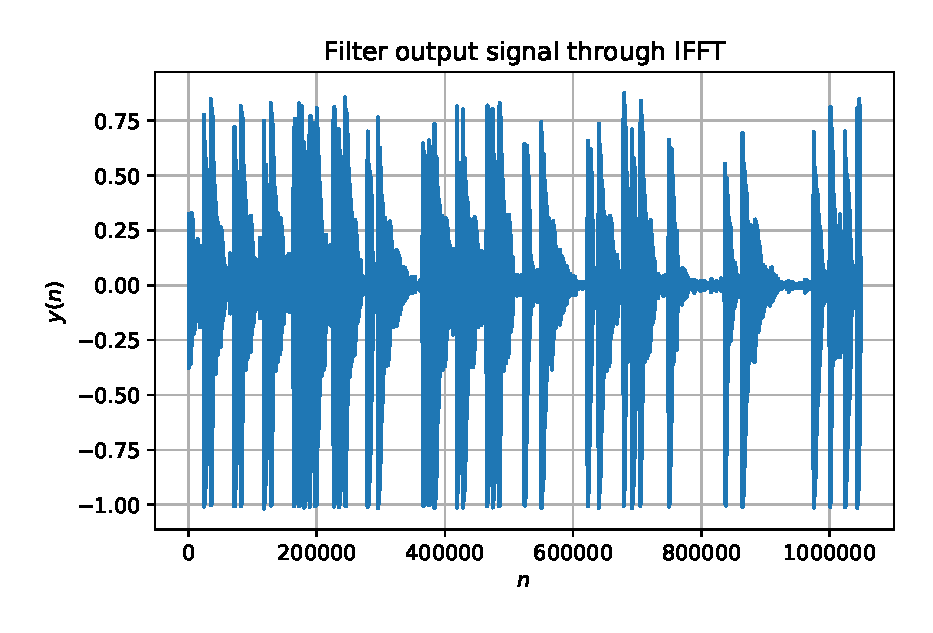
\includegraphics[width=\columnwidth]{./figs/ifft}
\caption{$y(n)$ from IFFT}
\label{fig:ifft}
\end{figure}
We can observe from the above plot that it is similar as the $y(n)$ observed in Fig.\ref{fig:xy}
\end{enumerate}


\end{document}
